\documentclass{beamer}
\usepackage{listings}
\usepackage[french]{babel}
\usepackage[utf8]{inputenc}
\usepackage[T1]{fontenc}
\usepackage{epsfig}
\usepackage{algorithm}
\usepackage{algorithmic}
\usepackage{fancybox}
\usepackage{amsmath}
\usepackage{latexsym}
\usepackage{amssymb}
\newcommand\rae{$\rightarrow$ }
\newenvironment{framentitle}[1]
{
\begin{frame}
  \frametitle{#1}
}
{
\end{frame}
}

\newcommand{\ra}{\rightarrow}
\newcommand{\fd}{\longrightarrow}
\newcommand{\fdd}{\longrightarrow}
\newcommand{\fgg}{\longleftarrow}
\usetheme{Singapore}
\setbeamercovered{transparent}
\setbeamertemplate{navigation symbols}{}
\setbeamertemplate{mini frames}{}
\title{UTC504 -- Systèmes d'Information et Bases de Données}
\subtitle{Conception d'une base de données -- MERISE}
\author{Sébastien Fourestier}
\date{2022}
%\setcounter{tocdepth}{1}

\lstset{
keywords={select,from,where,and,order,by,is,not,null,group,having,desc,union,
intersect,minus,or,as,distinct,insert,into,delete,values,commit,update,set,
inner,outer,full,join,cross,asc,count,on,using,natural,left,create,replace,
alter,user,identified,desc},
keywordstyle=\bfseries,         % bold keyword
%basicstyle=\small,
commentstyle=\itshape,          % default
stringstyle=\ttfamily,          % typewriter font for strings
tabsize=2,                      % indent
%numbers=left,                   % line numbers
%numberstyle=\tiny,              % line numbers size
stepnumber=2,                   % line numbers step
numbersep=5pt,                  % line numbers sep
inputencoding=utf8
%mathescape=false,               % math on listings
%extendedchars=true
}
%frame=single,                   % enable frame

\newenvironment{slide}[1]
{
  \begin{frame}\frametitle{#1}
}
{
  \end{frame}
}

\newcommand{\entete}
{
  \begin{frame}
  \titlepage
  \end{frame}
}

\newcommand{\plan}
{
  \begin{frame}
    \frametitle{Plan}
    \tableofcontents
  \end{frame}
}

%\newcommand{\currentplan}
%{
%  \begin{frame}
%    \frametitle{Plan}
%    \tableofcontents[currentsection]
%  \end{frame}
%}

%\AtBeginSubsection[]
\AtBeginSection[]
{
  \begin{frame}<beamer>
    \frametitle{Plan}
    \tableofcontents[currentsection]
%    \tableofcontents[currentsection,currentsubsection]
  \end{frame}
}

\begin{document}

\begin{frame}
\titlepage
\end{frame}

\plan
\section{Introduction}

\begin{frame}
  \frametitle{Bibliographie}
  \begin{itemize}
    \item Ce cours est très largement inspiré de celui de Cyril \textsc{Gruau} : Conception d'une base de
      données, \url{http://cyril-gruau.developpez.com/merise/}
    \item Il est également inspiré par les cours réalisés par des enseignants de
      l'ENSEIRB-MATMECA:\\A. Zemmari, M. Mosbah, B. Le Saëc
    \item Outil de réalisation de diagrammes entité-association : \url{http://www.analysesi.com/}
  \end{itemize}
\end{frame}

\begin{framentitle}{Correctifs}
    \begin{itemize}
        \item Ce cours est disponible sous licence libre sur ce dépôt github:\\
            \small{\url{https://github.com/sfourestier/enseignement}}
        \item[$\ra$] Voici pouvez :
            \begin{itemize}
                \item L'améliorer en proposant des \emph{Pull requests}
                \item Partager autour de points pouvant être améliorés en créant des
                    tickets (\emph{Issues})
            \end{itemize}
    \end{itemize}
\end{framentitle}

\begin{frame}
  \frametitle{Historique}
  \begin{itemize}
    \item Informatique :\\
      Construire des systèmes pour effectuer des calculs (équations différentielles, calcul matriciel, etc.)
    \item Aujourd'hui, on s'appuie de plus en plus sur des données $\ra$ gestion de grandes quantités d'informations:
      \begin{itemize}
        \item Stocker des données
        \item Manipuler ces données
      \end{itemize}
    \item Données de natures diverses, opérations plus ou moins compliquées
    \item[$\ra$] On se place donc dans le cas des systèmes d'informations de gestion
        \begin{itemize}
            \item Manipulent beaucoup de données
            \item[$\ra$] Modélisation de la manière dont les données seront
                organisées
        \end{itemize}
  \end{itemize}
\end{frame}

\begin{frame}
  \frametitle{Objectif d'un SGBD}
  \begin{itemize}
    \item Stocker, centraliser des données (BD) et les mettre à disposition des utilisateurs
    \item Manipuler (de manière transparente pour l'utilisateur) des données (SGBD)
    \item Exemples d'utilisation :
      \begin{itemize}
        \item Gestion : paye, stock, etc.
        \item Transactionnelles : banque, réservation, etc.
        \item Documentation : bibliothèque, cartographie, etc.
      \end{itemize}
  \end{itemize}
\end{frame}

\begin{frame}
  \frametitle{Fonctionnalités d'un SGBD (1)}
  \begin{itemize}
    \item Gestion du stockage :\\
      Tailles importantes des données, éviter les redondances
    \item Persistance :\\
      Les données survivent aux programmes qui les créent
    \item Fiabilité :\\
      Mécanismes de reprise sur pannes (logiciel ou matériel)
    \item Sécurité/Confidentialité :\\
      Contrôle des utilisateurs et des droits d'accès aux données
    \item Interfaces homme-machine :\\
      Ergonomie, profils utilisateurs
    \item Distribution :\\
      Données stockées sur différents sites
    \item Optimisation
  \end{itemize}
\end{frame}

\begin{frame}
\frametitle{Fonctionnalités d'un SGBD (2)}
\begin{itemize}
  \item Contrôle de concurrence : propriétés ACID, transactions
    \begin{itemize}
      \item Atomicité :\\
        Soit toutes les opérations de la transaction sont validées, soit aucune ne l'est
      \item Cohérence :\\
        Préservation de la cohérence de la base (contraintes d'intégrité, etc.)
      \item Isolation :\\
        Quelle que soit la manière dont les transactions concurrentes sont exécutées, on doit pouvoir les
        ordonner de sorte à ce que l'état final de la base soit le même qu'après une exécution séquentielle
        des différentes transactions.
    \item Durabilité :\\
      Si une transaction est validée, tous les changements qu'elle a effectués sur la base sont persistants
    \end{itemize}
\end{itemize}
\end{frame}

\begin{frame}
  \frametitle{Architecture fonctionnelle d'un SGBD}
  \begin{center}
    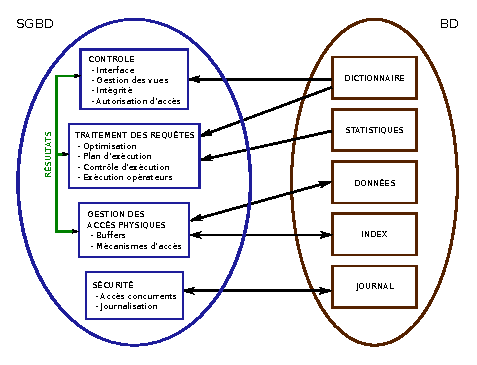
\epsfig{file=sgbd.eps,width=0.9\linewidth}
  \end{center}
\end{frame}

\begin{frame}
  \frametitle{Utilisateurs d'un SGBD}
  \begin{itemize}
    \item Administrateur
      \begin{itemize}
        \item Définition du schéma logique
        \item Définition des structures de stockage et les méthodes d'accès
        \item Gestion des autorisations
        \item Spécification des contraintes
        \item Maintenance de la performance
      \end{itemize}
    \item Concepteur et programmeur
      \begin{itemize}
        \item Est informaticien
        \item Connaît au moins le LMD
        \item Connaît bien le SGBD
        \item Connaît un ou plusieurs langages de programmation
      \end{itemize}
    \item Utilisateur
      \begin{itemize}
        \item Intervient en amont de la réalisation du SGBD
        \item Peut participer à la validation du schéma conceptuel
        \item Secrétariat, caissier, etc.
      \end{itemize}
  \end{itemize}
\end{frame}

\begin{frame}
  \frametitle{Niveau d'abstraction des données}
  \begin{center}
    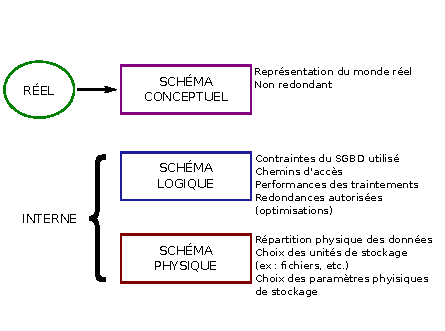
\includegraphics[width=\linewidth]{abstractions.pdf}
  \end{center}
\end{frame}

% \begin{frame}
%   \frametitle{Principes de base}
%   \begin{itemize}
%     \item Indépendance physique
%       \begin{itemize}
%         \item Les applications manipulant la base au niveau logique ne doivent pas être réécrites si la
%           structure physique est modifiée
%       \end{itemize}
%     \item Indépendance logique
%       \begin{itemize}
%         \item Une modification au niveau logique n'implique aucune modification des applications utilisant le
%           niveau externe
%       \end{itemize}
%     \item[$\ra$] Deux types de langages :
%       \begin{itemize}
%         \item Description des données (schéma)
%         \item Manipulation des données (instance) : requêtes et mise à jour
%       \end{itemize}
%   \end{itemize}
% \end{frame}

% \begin{frame}
%   \frametitle{Schéma et instance}
%   \begin{itemize}
%     \item Analogues à la notion de variable et de type dans les langages de programmation
%     \item Schéma : structure logique de la base de données
%       \begin{itemize}
%         \item Exemple : ensembles de clients, de produits et de fournisseurs
%       \end{itemize}
%     \item Instance : le contenu effectif de la base de données à un instant donné
%   \end{itemize}
% \end{frame}

\begin{frame}
  \frametitle{Modèles de données}
    On utilise la méthode MERISE :
  \begin{itemize}
    % \item Ensemble d'outils permettant de définir :
    %   \begin{itemize}
    %     \item Le schéma et les instances
    %     \item Les opérations possibles sur les instances
    %   \end{itemize}
    \item Modèle conceptuel de données :
      \begin{itemize}
        \item Entité-association
        \item (Diagramme de classes UML)
      \end{itemize}
    \item Modèle logique de données :
      \begin{itemize}
        \item Modèle relationnel
      \end{itemize}
    \item Modèle physique de données :
      \begin{itemize}
        \item Implémentation particulière du modèle logique de données par le logiciel
      \end{itemize}
  \end{itemize}
\end{frame}

\begin{frame}
  \frametitle{Conception d'une base de données}
  \begin{itemize}
    \item Conception d'une base de données:
      \begin{enumerate}
        \item Analyse des besoins
        \item Description conceptuelle
        \item Conception logique
        \item Conception physique
      \end{enumerate}
    \item Les 2 premières phases sont indépendantes du SGBD
    \item Le passage de 2 à 3 peut être en partie automatisé
  \end{itemize}
\end{frame}

\section[Modèle conceptuel]{Modèle conceptuel}

%\subsection{Définitions}

\begin{frame}
  \frametitle{Entité}
  \begin{itemize}
    \item Entité : population d'individus homogènes
  \end{itemize}
  \begin{center}
    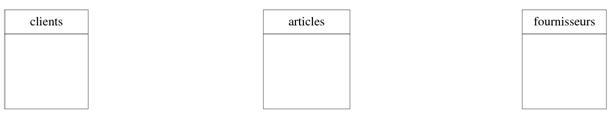
\includegraphics[width=0.9\linewidth]{entite.jpg}
  \end{center}
  \begin{itemize}
    \item Les produits ou les articles vendus par une entreprise sont de même nature (désignation, prix, etc.)
    \item[$\ra$] Ils peuvent être regroupés dans une même entité \emph{articles}
    \item Les \emph{articles} et les \emph{clients} ne sont pas de même nature (informations non homogènes)
    \item[$\ra$] On utilise deux entités distinctes
%      (un article ne possède pas d'adresse et un client ne possède pas de prix unitaire). Il
%      faut donc leur réserver deux entités distinctes : l'entité articles et l'entité clients.
  \end{itemize}
\end{frame}

\begin{frame}
  \frametitle{Association}
  \begin{itemize}
    \item Association : liaison qui a une signification précise entre plusieurs entités
  \end{itemize}
  \begin{center}
    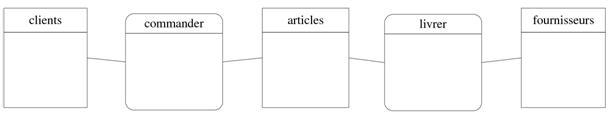
\includegraphics[width=0.9\linewidth]{association.jpg}
  \end{center}
  \begin{itemize}
    \item L'association \emph{commander} relie les entités \emph{articles} et \emph{clients}
    \item L'association \emph{livrer} relie les entités \emph{articles} et \emph{fournisseurs}
    \item L'entité \emph{clients} et relié indirectement à l'entité \emph{fournisseurs} via l'entité
      \emph{articles}
  \end{itemize}
\end{frame}

\begin{frame}
  \frametitle{Attribut}
  \begin{itemize}
    \item Attribut : propriété d'une entité ou d'une association
  \end{itemize}
  \begin{center}
    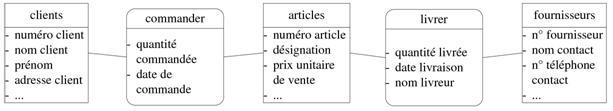
\includegraphics[width=0.9\linewidth]{attribut.jpg}
  \end{center}
  \begin{itemize}
    \item Le \emph{numéro article} et le \emph{prix unitaire} sont des attributs de l'entité \emph{articles},\\
      la \emph{quantité commandée} est un attribut de l'association \emph{commander}, etc.
    \item Une entité et ses attributs ne doivent traiter que d'un seul sujet
    \item[$\ra$] Mettre les informations relatives aux fournisseurs dans une entité \emph{fournisseurs} séparée
      plutôt que dans l'entité \emph{articles}
  \end{itemize}
\end{frame}

\begin{frame}
  \frametitle{Identifiant}
  \begin{itemize}
    \item Identifiant : attribut sans doublon qui identifie l'entité de manière unique
  \end{itemize}
  \begin{center}
    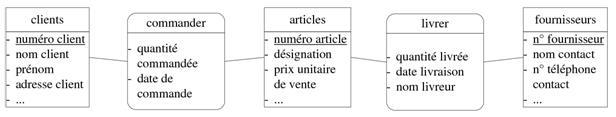
\includegraphics[width=0.9\linewidth]{identifiant.jpg}
  \end{center}
  \begin{itemize}
    \item Par convention, on souligne l'attribut identifiant sur le schéma
    \item En général, si il n'y a pas d'attribut adapté, on ajoute un numéro auto-incrémenté
    \item Une entité possède au moins un attribut (son identifiant)
    \item Une association peut être dépourvue d'attribut
  \end{itemize}
\end{frame}

%\subsection{Cardinalités}

\begin{frame}
  \frametitle{Cardinalités (1)}
  \begin{itemize}
    \item Cardinalité : pour un lien entre une entité et une association, elle précise le minimum et le maximum de
      fois qu'un individu de l'entité peut être concerné par l'association
  \end{itemize}
  \begin{center}
    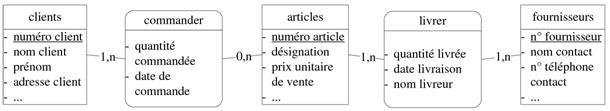
\includegraphics[width=0.9\linewidth]{cardinalites.jpg}
  \end{center}
  \begin{itemize}
    \item Exemple :
      \begin{itemize}
        \item Un \emph{client} a au moins commandé un \emph{article} et peut en commander $n$
        \item Un \emph{article} peut avoir été commandé entre $0$ et $n$ fois
      \end{itemize}
  \end{itemize}
\end{frame}

\begin{frame}
  \frametitle{Cardinalités (2)}
  \begin{center}
    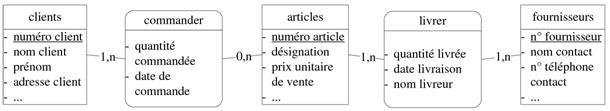
\includegraphics[width=0.9\linewidth]{cardinalites.jpg}
  \end{center}
  \begin{itemize}
    \item Une cardinalité minimale de $0$ : les individus de l'entité peuvent exister seuls
    \item Une cardinalité minimale de $1$ : les individus de l'entité ont besoin de l'association pour exister
      (un client n'existe que si il a commandé)
    \item Une cardinalité maximale de $1$ : les individus de l'entité sont reliés au maximum à un autre individu
      de l'autre entité
    \item Une cardinalité maximale de $n$ : les individus de l'entité peuvent reliés à plusieurs individus de
      l'autre entité
    \item En général, on n'utilise pas de cardinalités minimales de plus de $1$ car elle n'auront pas d'impact
      par la suite (cf. modèle relationnel)
  \end{itemize}
\end{frame}

%\subsection{Associations}

\begin{frame}
  \frametitle{Associations plurielles}
  \begin{itemize}
    \item Deux mêmes entités peuvent être plusieurs fois en association
  \end{itemize}
  \begin{center}
    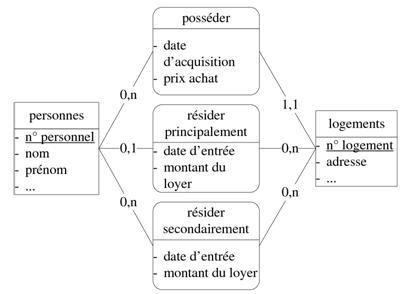
\includegraphics[width=0.6\linewidth]{associations_plurielles.jpg}
  \end{center}
  \begin{itemize}
    \item Permet d'indiquer des liens de différentes natures
  \end{itemize}
\end{frame}

\begin{frame}
  \frametitle{Association réflexive}
  \begin{itemize}
    \item Une association peut être reliée plusieurs fois avec la même entité
  \end{itemize}
  \begin{center}
    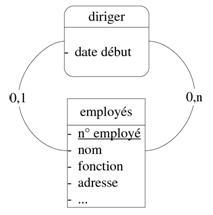
\includegraphics[width=0.35\linewidth]{association_reflexive.jpg}
  \end{center}
  \begin{itemize}
    \item Un employé est dirigé par un autre employé (sauf le directeur général)
    \item Un employé peut diriger plusieurs autres employés
  \end{itemize}
\end{frame}

\begin{frame}
  \frametitle{Associations non binaires (1)}
  \begin{itemize}
    \item Une entité avec associations de cardinalités maximales 1 au centre et n à l'extérieur peut-être
      remplaçée par une association avec les cardinalités extérieures
  \end{itemize}
  \begin{center}
    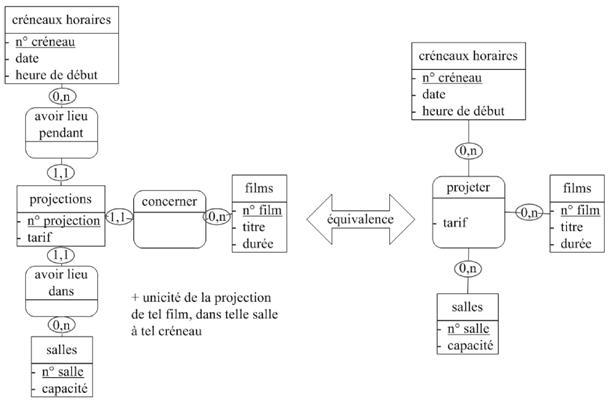
\includegraphics[width=0.8\linewidth]{assocation_ternaire.jpg}
  \end{center}
\end{frame}

\begin{frame}
  \frametitle{Associations non binaires (2)}
  \begin{itemize}
    \item Passer par un schéma entités-associations avec des associations binaires dans un premier temps
      permet d'éviter les association $n$-aires abusives (cardinalités non adéquates)
  \end{itemize}
  \begin{center}
    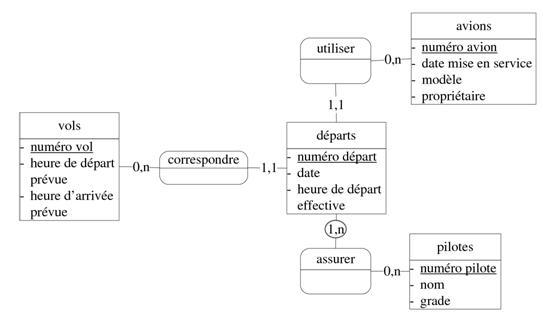
\includegraphics[width=0.8\linewidth]{assocation_ternaire2.jpg}
  \end{center}
\end{frame}

\begin{frame}
  \frametitle{Associations non binaires (3)}
  \begin{itemize}
    \item Une association peut être branchée à plus de trois entités
  \end{itemize}
  \begin{center}
    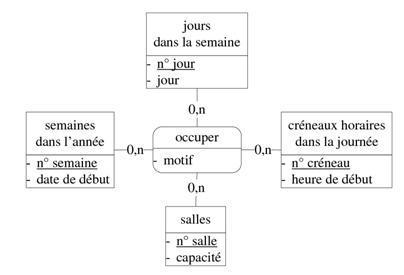
\includegraphics[width=0.6\linewidth]{assocation_quaternaire.jpg}
  \end{center}
\end{frame}

\begin{frame}
  \frametitle{Méthodologie}
  \begin{enumerate}
    \item Identifier les entités en présence
    \item Lister leurs attributs
    \item Ajouter les identifiants
    \item Établir les associations binaires entre les entités
    \item Lister leurs attributs
    \item Calculer les cardinalités
    \item Vérifier les règles de normalisation
    \item Effectuer les corrections nécessaires
  \end{enumerate}
\end{frame}

\section[Normalisation]{Normalisation}

%\subsection{Règles de normalisations}

\begin{frame}
  \frametitle{Bonnes pratiques}
  \begin{itemize}
    \item Un bon schéma entités-associations doit répondre à 9 règles de normalisation:
      \begin{enumerate}
        \item Normalisation des entités
        \item Normalisation des noms
        \item Normalisation des identifiants
        \item Normalisation des attributs
        \item Normalisation des associations
        \item Normalisation des cardinalités
        \item Première forme normale
        \item Deuxième forme normale
        \item Troisième forme normale
      \end{enumerate}
  \end{itemize}
\end{frame}

\begin{frame}
  \frametitle{Normalisation des entités}
  \begin{itemize}
    \item Toutes les entités qui sont remplaçables par une association doivent être remplacées
  \end{itemize}
\end{frame}


\begin{frame}
  \frametitle{Normalisation des noms (1)}
  \begin{itemize}
    \item Le nom d'une entité, d'une association ou d'un attribut doit être unique
    \item Conseils :
      \begin{itemize}
        \item Pour les entités, utiliser un nom commun au pluriel (ex : clients)
        \item Pour les associations, utiliser un verbe à l'infinitif (ex : effectuer, concerner)
          éventuellement à la forme passive (être commandé) et accompagné d'un adverbe (avoir lieu dans,
          pendant, à)
        \item Pour les attributs, utiliser un nom commun singulier (ex : nom, numéro, libellé,
          description), éventuellement accompagné du nom de l'entité ou de l'association dans laquelle il se
          trouve (ex : nom de client, numéro d'article)
      \end{itemize}
    \item Remarque : lorsqu'il reste plusieurs fois le même nom, c'est parfois symptomatique d'une modélisation qui
      n'est pas terminée
  \end{itemize}
\end{frame}

\begin{frame}
  \frametitle{Normalisation des noms (2)}
  \begin{itemize}
    \item Deux entités homogènes peuvent être fusionnées
  \end{itemize}
  \begin{center}
    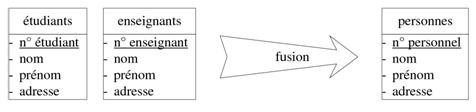
\includegraphics[width=0.8\linewidth]{fusion_entites.jpg}
  \end{center}
\end{frame}

\begin{frame}
  \frametitle{Normalisation des noms (3)}
  \begin{itemize}
    \item Éviter les redondances : gaspillage d'espace et risque incohérence
  \end{itemize}
  \begin{center}
    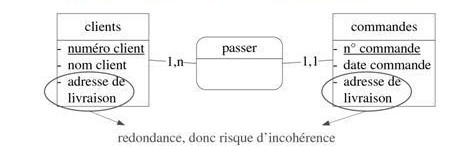
\includegraphics[width=0.8\linewidth]{redondance_attributs.jpg}
  \end{center}
  \begin{itemize}
    \item Si les adresses ne sont pas les mêmes, où faut-il livrer ?
  \end{itemize}
\end{frame}

\begin{frame}
  \frametitle{Normalisation des identifiants}
  \begin{itemize}
    \item Chaque entité doit posséder un identifiant
    \item Conseils :
      \begin{itemize}
        \item Éviter les identifiants composés de plusieurs attributs (ex : nom et prénom) : mauvaises
          performances et problème d'unicité possible
        \item Préférer un identifiant court pour une recherche plus rapide (éviter notamment les chaînes de
          caractères complexes)
        \item Éviter les identifiants susceptibles de changer au cours du temps (ex : les plaques d'immatriculation)
      \end{itemize}
    \item Conclusion : en général, l'identifiant est un entier, souvent incrémenté automatiquement
  \end{itemize}
\end{frame}

\begin{frame}
  \frametitle{Normalisation des attributs (1)}
  \begin{itemize}
    \item Remplacer les attributs en plusieurs exemplaires en une association supplémentaire de cardinalités
      maximales $n$
  \end{itemize}
  \begin{center}
    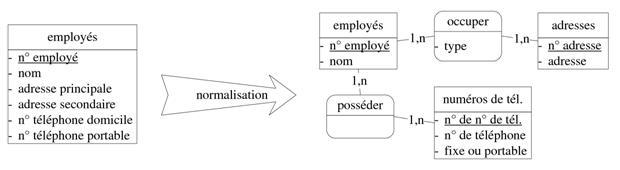
\includegraphics[width=0.9\linewidth]{normalisation_attributs.jpg}
  \end{center}
  \begin{itemize}
    \item Problème d'évolutivité des attributs en plusieurs exemplaires : comment faire si un employé a deux
      adresses secondaires ?
  \end{itemize}
\end{frame}

\begin{frame}
  \frametitle{Normalisation des attributs (2)}
  \begin{itemize}
    \item Ne pas avoir d'attribut calculable à partir d'autres attributs
  \end{itemize}
  \begin{center}
    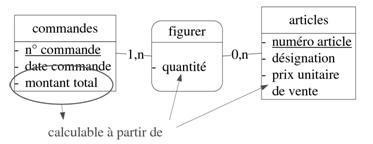
\includegraphics[width=0.6\linewidth]{attribut_calculable.jpg}
  \end{center}
  \begin{itemize}
    \item Risque d'incohérence entre les valeurs des attributs de base et celles des attributs calculés
    \item Attributs calculables classiques à éviter:
      \begin{itemize}
        \item l'âge : calculable à partir de la date de naissance
        \item le département : calculable à partir du code postal
      \end{itemize}
  \end{itemize}
\end{frame}

\begin{frame}
  \frametitle{Normalisation des attributs des associations (1)}
  \begin{itemize}
    \item Les attributs d'une association doivent dépendre directement des identifiants de toutes les entités
      en association
  \end{itemize}
  \begin{center}
    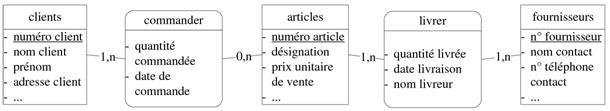
\includegraphics[width=0.9\linewidth]{cardinalites.jpg}
  \end{center}
  \begin{itemize}
    \item La quantité commandée dépend de numéro de client et du numéro d'article, la date de commande non
    \item[$\ra$] Création d'une entité commandes (idem pour les livraisons)
  \end{itemize}
\end{frame}

\begin{frame}
  \frametitle{Normalisation des attributs des associations (2)}
  \begin{itemize}
    \item Les attributs d'une association doivent dépendre directement des identifiants de toutes les entités
      en association
  \end{itemize}
  \begin{center}
    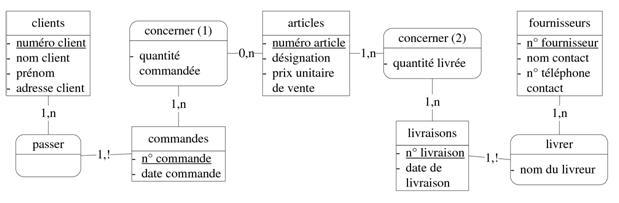
\includegraphics[width=0.9\linewidth]{normalisation_attributs_associations.jpg}
  \end{center}
  \begin{itemize}
    \item La quantité commandée dépend de numéro de client et du numéro d'article, la date de commande non
    \item[$\ra$] Création d'une entité commandes (idem pour les livraisons)
  \end{itemize}
\end{frame}

\begin{frame}
  \frametitle{Normalisation des attributs des associations (3)}
  \begin{itemize}
    \item Une entité avec une cardinalité de 1,1 ou 0,1 aspire les attributs de l'association
  \end{itemize}
  \begin{center}
    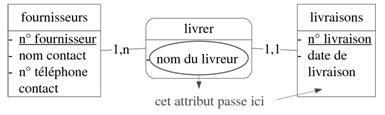
\includegraphics[width=0.6\linewidth]{normalisation_attribut_association.jpg}
  \end{center}
\end{frame}

\begin{frame}
  \frametitle{Normalisation des associations (1)}
  \begin{itemize}
    \item On élimine les associations fantômes, redondantes ou en plusieurs exemplaires
  \end{itemize}
  \begin{center}
    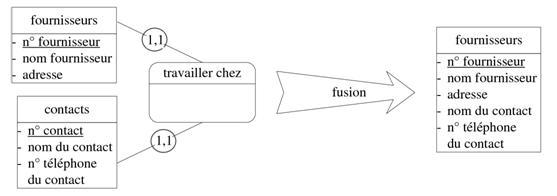
\includegraphics[width=0.9\linewidth]{association_fantome.jpg}
  \end{center}
  \begin{itemize}
    \item Les cardinalités sont toutes 1,1 donc c'est une association fantôme
  \end{itemize}
\end{frame}

\begin{frame}
  \frametitle{Normalisation des associations (2)}
  \begin{itemize}
    \item Les associations redondantes signifient qu'il existe deux chemins pour aller d'une entité à une autre :
      \begin{itemize}
        \item Ils doivent avoir deux significations ou deux durées de vie différentes
        \item Ou le chemin le plus court doit être supprimé
      \end{itemize}
  \end{itemize}
  \begin{center}
    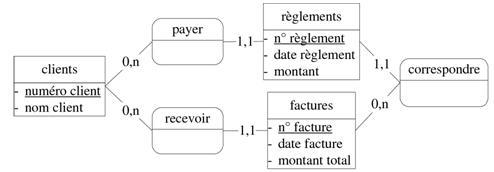
\includegraphics[width=0.9\linewidth]{association_redondante.jpg}
  \end{center}
  \begin{itemize}
    \item Si un client ne peut pas régler la facture d'un autre client, alors l'association payer est inutile
    \item[$\ra$] Elle doit être supprimée
  \end{itemize}
\end{frame}

\begin{frame}
  \frametitle{Normalisation des associations (3)}
  \begin{itemize}
    \item Les associations en plusieurs exemplaires doivent, si elle le peuvent, être regroupée
      \begin{itemize}
        \item Évolutivité : on privilégie les cardinalités maximales $n$
        \item Une cadinalité minimale de plus de $1$ est inutile si la cardinalité maximale est $n$
      \end{itemize}
  \end{itemize}
  \begin{center}
    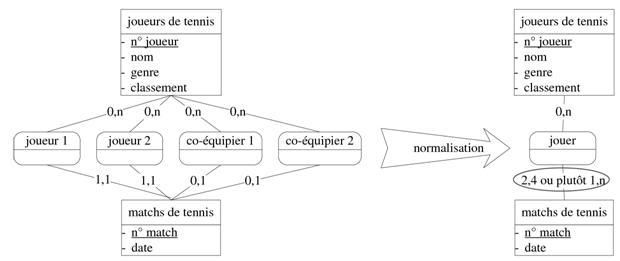
\includegraphics[width=0.9\linewidth]{association_plusieurs_exemplaires.jpg}
  \end{center}
  \begin{itemize}
    \item Une association suffit pour remplacer les 4 associations
  \end{itemize}
\end{frame}

%\subsection{Les formes normales}

\begin{frame}
  \frametitle{Première forme normale}
  \begin{itemize}
    \item Tous les attributs doivent posséder une valeur sémantiquement
        atomique.
    \item Conséquence : à un instant donné un attribut ne peut prendre qu'une
        valeur et non pas, un ensemble ou une liste de valeurs
  \end{itemize}
  \begin{center}
    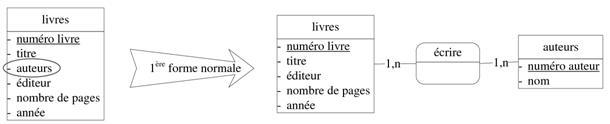
\includegraphics[width=0.9\linewidth]{premiere_forme_normale.jpg}
  \end{center}
  \begin{itemize}
    \item Si un attribut prend plusieurs valeurs, alors ces valeurs doivent faire l'objet d'une entité
      supplémentaire, en association avec la première
  \end{itemize}
\end{frame}

\begin{frame}
  \frametitle{Deuxième forme normale}
  \begin{itemize}
    \item «~En première forme normale et :\\
        Un attribut non identifiant ne dépend pas d’une partie de l'identifiant
        mais de tout l'identifiant~»
    \item Cela peut arriver si l'identifiant est composé de plusieurs attributs
    \item[$\ra$] Peut être oubliée si l'on utilise des identifiants non composés et de type entier
  \end{itemize}
\end{frame}

\begin{frame}
  \frametitle{Troisième forme normale}
  \begin{itemize}
    \item «~En deuxième forme normale et :\\
        Tous les attributs non identifiants doivent dépendre directement de
        l'identifiant~»
    \item En pratique on utilise la troisième forme normale de Boyce-Codd, plus complète
  \end{itemize}
\end{frame}

\begin{frame}
  \frametitle{Troisième forme normale de Boyce-Codd (1)}
  \begin{itemize}
    \item «~En deuxième forme normale et :
        \begin{itemize}
            \item Tous les attributs non identifiants doivent dépendre directement de l'identifiant
            \item Aucune partie de l'identifiant dépend d'un attribut
                non-identifiant~»
        \end{itemize}
  \end{itemize}
\end{frame}

\begin{frame}
  \frametitle{Troisième forme normale de Boyce-Codd (2)}
  \begin{itemize}
    \item Version simplifié : tous les attributs d'une entité doivent dépendre directement de son identifiant
      et d'aucun autre attribut
    \item Si ce n'est pas le cas, il faut placer l'attribut pathologique dans une entité séparée en
      association avec la première
  \end{itemize}
  \begin{tabular}{c | c | c | c | c }
    numéro avion & constructeur & modèle & capacité & propriétaire \\
    \hline \hline
    1 & Airbus & 380 & 180 & Air France \\
    2 & Boeing & 747 & 314 & British Airways \\
    3 & Airbus & 380 & 180 & KLM
  \end{tabular}
  \begin{itemize}
    \item Redondance ($\ra$ risque d'incohérence) pour les colonnes constructeur
        et capacité qui dépendent de modèle
  \end{itemize}
\end{frame}

\begin{frame}
  \frametitle{Troisième forme normale de Boyce-Codd (3)}
  \begin{itemize}
    \item Version simplifié : tous les attributs d'une entité doivent dépendre directement de son identifiant et d'aucun autre
      attribut
    \item Si ce n'est pas le cas, il faut placer l'attribut pathologique dans une entité séparée en
      association avec la première
  \end{itemize}
  \begin{center}
    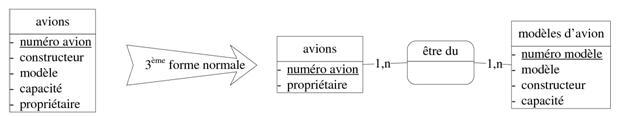
\includegraphics[width=0.9\linewidth]{troisieme_forme_normale.jpg}
  \end{center}
  \begin{itemize}
    \item La colonne constructeur devrait également être dans une entité séparée constructeurs (en association avec modèles d'avion)
  \end{itemize}
\end{frame}


\section{Dépendances fonctionnelles}

%\subsection{Définitions}
\begin{frame}
  \frametitle{Dépendances fonctionnelles}
  \begin{itemize}
    \item Méthode pour établir efficacement un modèle entités-associations bien normalisé:
      \begin{enumerate}
        \item Étudier les dépendances fonctionnelles
        \item Obtention du graphe de couverture minimale
        \item Traduction du graphe en modèle
      \end{enumerate}
    \item Traditionnellement employé pour normaliser des modèles relationnels
  \end{itemize}
\end{frame}

\begin{frame}
  \frametitle{Définition}
  \begin{itemize}
    \item Un attribut $B$ dépend fonctionnellement d'un attribut $A$ si et seulement si une valeur de $A$ induit une
      unique valeur de $B$
    \item On note une dépendance fonctionnelle par une flèche simple : $$A \ra B$$
  \end{itemize}
\end{frame}

\begin{frame}
  \frametitle{Transitivité}
  \begin{itemize}
    \item Une dépendance fonctionnelle est transitive : $$\text{si } A \ra B \text{ et } B \ra C \text{ alors } A \ra C$$
    \item Exemple:\\
      si \emph{numéro commande} $\ra$ \emph{numéro client} $\ra$ \emph{nom client}\\
      alors \emph{numéro commande} $\ra$ \emph{nom client}
    \item Deux types de dépendances fonctionnelles :
      \begin{itemize}
        \item directe: \emph{numéro commande} $\ra$ \emph{numéro client}
        \item transitive: \emph{numéro commande} $\ra$ \emph{nom client}
      \end{itemize}
  \end{itemize}
\end{frame}

\begin{frame}
  \frametitle{Dépendances fonctionnelles non élémentaires}
  \begin{itemize}
    \item Dépendance fonctionnelles non élémentaire :\\
      Un attribut $B$ a une dépendance fonctionnelle qui repose sur la conjonction de plusieurs
      attributs
    \item On note une dépendance fonctionnelle non élémentaire par une flèche unique avec plusieurs points
      d'entrée (regroupés autour d'un cercle)
  \end{itemize}
  \begin{center}
    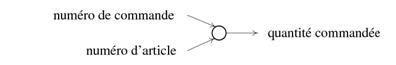
\includegraphics[width=0.9\linewidth]{dependance_fonctionnelle_non_elementaire.jpg}
  \end{center}
  \begin{itemize}
  \item Dans l'exemple, dépendance fonctionnelle à la fois non élémentaire et directe
  \end{itemize}
\end{frame}

\begin{frame}
  \frametitle{Graphe de couverture minimale}
  \begin{itemize}
    \item Graphe de couverture minimale :\\
      Réseau obtenu en représentant tous les attributs et toutes les dépendances fonctionnelles directes entre
      ces derniers
  \end{itemize}
  \begin{center}
    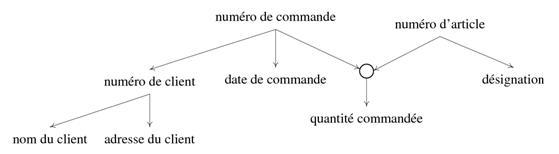
\includegraphics[width=0.9\linewidth]{graphe_couverture_minimale.jpg}
  \end{center}
\end{frame}

\begin{framentitle}{Clé}
    Soit une relation $R$ avec ${A_1, \dots, A_n}$ attributs.

    Soit $X$ un sous-ensemble d'attributs de $R$, $X$ est une clé ou un
    identifiant si :
    \begin{itemize}
        \item Pour tous les attributs $A_i$ de $R$, $X \ra A_i$
        \item $X$ est le plus petit élément qui détermine tous les autres,
            c'est-à-dire, il n'existe pas $Y$ un sous-ensemble $X$ avec pour
            tous les attributs de $A_i$ de $R$, $X \ra A_i$
    \end{itemize}
\end{framentitle}

%\subsection{Méthodologie}
\begin{frame}
  \frametitle{Méthodologies}
  \begin{itemize}
    \item Nous avons vu à la fin de la section \og Modèle conceptuel \fg\ une méthodologie pour obtenir un
      modèle conceptuel de donnée
    \item Nous allons maintenant voir une méthodologie à partir de l'étude des dépendances fonctionnelles
      directes
  \end{itemize}
\end{frame}

\begin{frame}
  \frametitle{Méthodologie classique}
  \begin{enumerate}
    \item Identifier les entités en présence
    \item Lister leurs attributs
    \item Ajouter les identifiants
    \item Établir les associations binaires entre les entités
    \item Lister leurs attributs
    \item Calculer les cardinalités
    \item Vérifier les règles de normalisation, en particulier:
      \begin{itemize}
        \item Normalisation des entités (associations non binaires, etc.)
        \item Normalisation des associations et des attributs
        \item Troisième forme normale de Boyce-Codd
      \end{itemize}
    \item Effectuer les corrections nécessaires
  \end{enumerate}
\end{frame}

\begin{frame}
  \frametitle{Traduction à partir des dépendances fonctionnelles}
  \begin{itemize}
    \item Plusieurs étapes pour passer du graphe de couverture minimale à un schéma entités-associations normalisé
  \end{itemize}
  \begin{center}
    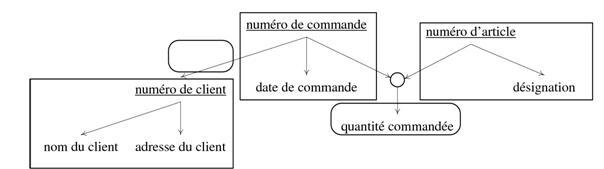
\includegraphics[width=0.9\linewidth]{graphe_identifie_5.jpg}
  \end{center}
\end{frame}

\begin{frame}
  \frametitle{Étapes de traduction (1)}
  \begin{center}
    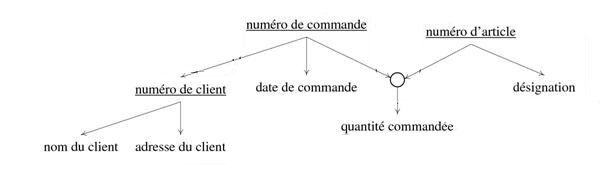
\includegraphics[width=0.9\linewidth]{graphe_identifie_1.jpg}
  \end{center}
  \begin{itemize}
    \item Étape 1 : repérer et souligner les identifiants (choisir les clés)
  \end{itemize}
\end{frame}

\begin{frame}
  \frametitle{Étapes de traduction (2)}
  \begin{center}
    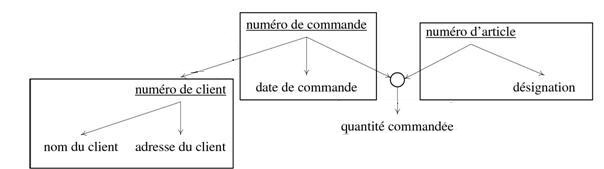
\includegraphics[width=0.9\linewidth]{graphe_identifie_2.jpg}
  \end{center}
  \begin{itemize}
    \item Étape 2 : tous les attributs non identifiant qui dépendent directement d'un identifiant et d'un
      seul, forment (avec l'identifiant) une entité
  \end{itemize}
\end{frame}

\begin{frame}
  \frametitle{Étapes de traduction (3)}
  \begin{center}
    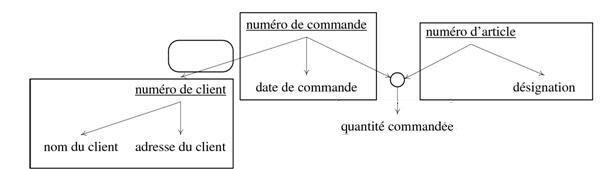
\includegraphics[width=0.9\linewidth]{graphe_identifie_3.jpg}
  \end{center}
  \begin{itemize}
    \item Étape 3 : les dépendances élémentaires entre les identifiants forment des associations
      binaires dont les cardinalités maximales sont $1$ au départ de la dépendance fonctionnelle et $n$ à
      l'arrivée
  \end{itemize}
\end{frame}

\begin{frame}
  \frametitle{Étapes de traduction (4)}
  \begin{center}
    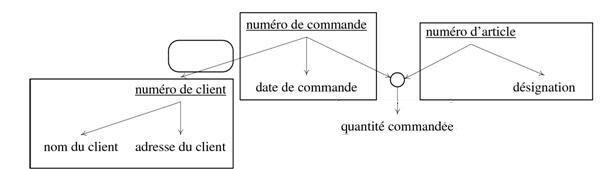
\includegraphics[width=0.9\linewidth]{graphe_identifie_3.jpg}
  \end{center}
  \begin{itemize}
    \item Étape 4 : sauf si entre deux identifiants se trouvent deux dépendances élémentaires réflexives,
      auquel cas l'association binaire a deux cardinalités maximales valant $1$
  \end{itemize}
\end{frame}

\begin{frame}
  \frametitle{Étapes de traduction (5)}
  \begin{center}
    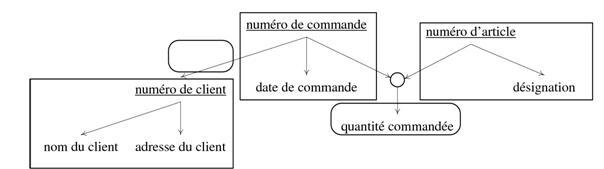
\includegraphics[width=0.9\linewidth]{graphe_identifie_5.jpg}
  \end{center}
  \begin{itemize}
    \item Étape 5 : les attributs (non identifiants) qui dépendent de plusieurs identifiants sont les
      attributs d'une association supplémentaire dont les cardinalités maximales sont toutes $n$
  \end{itemize}
\end{frame}

\begin{frame}
  \frametitle{Schéma obtenu}
  \begin{center}
    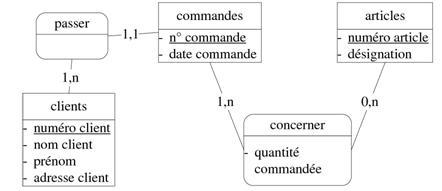
\includegraphics[width=0.9\linewidth]{schema_traduit.jpg}
  \end{center}
\end{frame}

\begin{frame}
  \frametitle{Remarques}
  \begin{itemize}
    \item Il faut donner un nom aux entités et aux associations
    \item Il reste les cardinalités minimales à établir
    \item En pratique, il faut connaître les entités pour établir le graphe de couverture minimale
    \item[$\ra$] Aide surtout à:
      \begin{itemize}
        \item Établir les associations entre les entités
        \item Normaliser les entités et leurs associations jusqu'en troisième forme normale de Boyce-Codd 
      \end{itemize}
  \end{itemize}
\end{frame}

\begin{frame}
  \frametitle{Méthodologie avec dépendances fonctionnelles}
  \begin{itemize}
    \item Identifier les entités et leur donner un identifiant
    \item Ajouter les attributs et leur dépendances fonctionnelles directes avec les identifiants
      (commencer par les dépendances élémentaires)
    \item Traduire le graphe de couverture minimale obtenu en un schéma entités-associations
    \item Ajuster les cardinalités minimales
    \item La majorité des règles de normalisation devraient être vérifiées, vérifier notamment:
      \begin{itemize}
        \item La normalisation des noms
        \item Les attributs en plusieurs exemplaires
        \item Les associations redondantes ou en plusieurs exemplaires
      \end{itemize}
  \end{itemize}
\end{frame}

% \begin{frame}
%   \frametitle{Remarques}
%   \begin{itemize}
%     \item Le modèle doit :
%       \begin{itemize}
%         \item Être \emph{exhaustif} : contenir toutes les informations nécessaires
%         \item Éviter les \emph{redondances} : perte d'espace, plus de travail de maintenance, risque d'incohérence
%       \end{itemize}
%     \item Ces méthodologies sont plutôt utilisées itérativement pour converger vers une modélisation
%       pertinente
%   \end{itemize}
% \end{frame}

%\subsection{Cas particuliers}
\begin{frame}
  \frametitle{Gestion des dates et de l'historique (1)}
  \begin{itemize}
    \item Dans une bibliothèque, on peut vouloir stocker les emprunts en cours ou les emprunts historiques
  \end{itemize}
  \begin{center}
    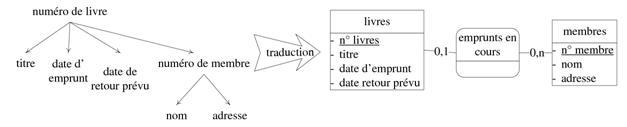
\includegraphics[width=0.9\linewidth]{emprunts_en_cours.jpg}
  \end{center}
  \begin{itemize}
    \item Emprunts en cours : la date de retour prévu est un attribut de l'entité livres car un livre
      ne peut faire l'objet que d'un seul emprunt en cours
  \end{itemize}
\end{frame}

\begin{frame}
  \frametitle{Gestion des dates et de l'historique (2)}
  \begin{itemize}
    \item Emprunts historiques :
      \begin{itemize}
        \item Un livre peut faire l'objet de plusieurs emprunts historiques
        \item Date d'emprunt est nécessaire pour connaître la date de retour prévue
        \item On évite d'avoir une date comme identifiant
        \item Une dépendance fonctionnelle ne peut partir que d'un ou plusieurs identifiant(s)
      \end{itemize}
    \item[$\ra$] C'est le signe qu'il manque un identifiant : le numéro d'emprunt
  \end{itemize}
\end{frame}

\begin{frame}
  \frametitle{Gestion des dates et de l'historique (3)}
  \begin{center}
    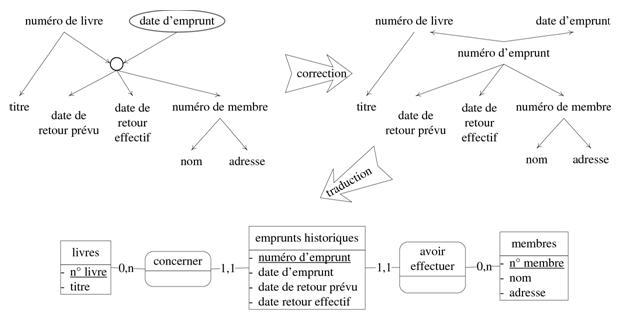
\includegraphics[width=0.9\linewidth]{gestion_historique.jpg}
  \end{center}
\end{frame}

\begin{frame}
  \frametitle{Gestion des dates et de l'historique (4)}
  \begin{itemize}
    \item Même pour une entité historisée, il vaut mieux éviter que la date n'entre dans l'identifiant
    \item Ici, l'entité emprunts historiques ne peut pas être transformée en une association (normalisation
      des attributs des associations) :\\ date retour effectif ne dépend pas du numéro de livre et du numéro de membre, mais du numéro de livre et de la date
      d'emprunt
    % \item La normalisation des entités ne s'applique donc pas aux entités qui ont un caractère historique
    \item[$\ra$] Si il n'y avait que le numéro et la date d'emprunt, on pourrait
        utiliser une association
  \end{itemize}
\end{frame}

\begin{frame}
  \frametitle{Dépendances plurielles}
  \begin{itemize}
    \item Une ou plusieurs dépendances fonctionnelles partent ou arrivent plusieurs fois du même
      attribut
  \end{itemize}
  \begin{center}
    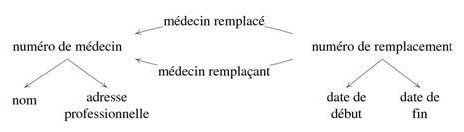
\includegraphics[width=0.9\linewidth]{dependances_plurielles.jpg}
  \end{center}
  \begin{itemize}
    \item Ajouter un commentaire sur la flèche permet de clarifier la signification de chaque dépendance
    \item Ce commentaire donnera le nom des associations correspondantes
    \item Dépendances fonctionnelles entre médecins et remplacements\\$\ra$ associations plurielles entre entités médecins et remplacements
  \end{itemize}
\end{frame}

\begin{frame}
  \frametitle{Dépendances réflexives}
  \begin{itemize}
    \item Dépendances fonctionnelles réflexives : $X \ra X$
  \end{itemize}
  \begin{center}
    
\includegraphics[width=0.9\linewidth]{dependances_reflexives.jpg}
  \end{center}
  \begin{itemize}
    \item Intérêt : seulement si elles ont une signification particulière
  \end{itemize}
\end{frame}

\begin{frame}
  \frametitle{Associations sans attributs}
  \begin{itemize}
    \item Attention : associations avec cardinalités maximales $n$ et sans attribut ne figurent pas sur le
      graphe de couverture minimale
  \end{itemize}
  \begin{center}
    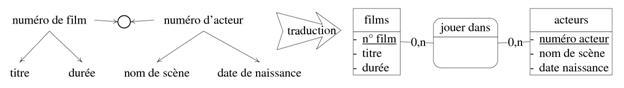
\includegraphics[width=\linewidth]{association_sans_attribut.jpg}
  \end{center}
  \begin{itemize}
    \item Possiblilité d'introduire une notation spéciale
    \item Exemple: une dépendance non élémentaire qui ne débouche sur aucun attribut
  \end{itemize}
\end{frame}

\section[Modèle relationnel]{Modèle relationnel}

%\subsection{Historique et définitions}

\begin{frame}
  \frametitle{Systèmes logiques : historique}
  \begin{itemize}
    \item Fichiers binaires et gérées par des programmes exécutables : modification de la structure des données très problématique
    \item SGBD hiérarchiques : Données organisées en arbre
    \item SGBD réseaux : Données organisées en graphe
    \item SGBD hiérarchiques et réseaux : dit navigationnels car on peut retrouver l'information à
      partir du chemin d'accès
    \item Pour chacun de ces systèmes, il existe des méthodes de traductions du MLD vers le MPD 
  \end{itemize}
\end{frame}

\begin{frame}
  \frametitle{Systèmes logiques : historique (2)}
  \begin{itemize}
    \item SGBD relationnels (SGBDR) : Information obtenue avec langage quasiment naturel (SQL pour
      Structured Query Langage)
    \item SGBD orientés objets : Il existe des \emph{framework} avec des \emph{mapping} objet-relationnel
      (\emph{ORM})
    \item Les bases de données NoSQL
      \begin{itemize}
        \item Relachement des propriétés ACID
        \item Permet la gestion d'un très grand nombre de données\\(\emph{Big Data})
      \end{itemize}
    \item Pour ce cours : modèle logique relationnel, abrégé:\\\og modèle relationnel \fg
  \end{itemize}
\end{frame}

\begin{frame}
  \frametitle{Modèle logique de données}
  \begin{itemize}
    \item Le modèle logique de données propose une modélisation plus concrète 
    \item Il est proche du modèle physique de données (qui sera implémenté)
    \item Il peut être traduit directement depuis le modèle conceptuel de données
  \end{itemize}
\end{frame}

\begin{frame}
  \frametitle{Tables, lignes et colonnes}
  \begin{itemize}
    \item Table : regroupe les données qui ont la même structure
    \item Colonne : décrit les champs en commun
    \item Ligne : contient les valeurs de ces champs pour un enregistrement
    \item Les lignes d'une table doivent être uniques
  \end{itemize}
  \begin{tabular}{c | c | c | c}
    numéro client & nom & prénom & adresse \\
    \hline \hline
    1 & Dupont & Michel & 127, rue\ldots \\
    2 & Durand & Jean & 314, boulevard\ldots \\
    3 & Dubois & Claire & 51, avenue\ldots \\
    4 & Dupuis & Marie & 2, impasse\ldots \\
    \ldots & \ldots & \ldots & \ldots
  \end{tabular}
  \begin{itemize}
    \item Exemple : table des renseignements clients
  \end{itemize}
\end{frame}

\begin{frame}
  \frametitle{Clés primaires}
  \begin{itemize}
    \item Clé primaire :
        \begin{itemize}
            \item Ensemble des colonnes permettant d'identifier une ligne
        \end{itemize}
    \item Une clé primaire ne peut avoir la valeur vide (NULL)
    \item La valeur de la clé primaire ne devrait pas changer au cours du temps
  \end{itemize}
\end{frame}

\begin{frame}
  \frametitle{Clés étrangères}
  \begin{itemize}
    \item Une colonne Colonne1 d'une table est clé étrangère ou référence la
        colonne Colonne2, si :
        \begin{itemize}
            \item Si elle ne contient que des valeurs prises par la colonne
                Colonne2 d'une autre table
            \item Colonne2 est sans doublons
        \end{itemize}
    \item Par convention, on souligne les clés primaires et on fait précéder les clés étrangères d'un dièse \#
      dans la description des colonnes d'une table :
    \item \texttt{clients(\underline{numéro client}, nom client, prénom, adresse client)}
    \item \texttt{commandes(\underline{numéro commande}, date de commande, \#numéro client (non vide))}
  \end{itemize}
\end{frame}

\begin{frame}
  \frametitle{Remarques}
  \begin{itemize}
    \item Une même table peut avoir plusieurs clés étrangères mais une seule clé primaire
    \item Une clé étrangère peut aussi être primaire (dans la même table)
    \item Une clé étrangère peut être composée (c'est le cas si la clé primaire référencée est composée)
    \item Chaque colonne qui compose une clé primaire ne peut pas recevoir la valeur vide (NULL)
%    \item Il est possible de préciser en SQL qu'une colonne doit pas recevoir la valeur vide (cf. suite du
%      cours)
%    \item Les SGBDR vérifient que chaque clé étrangère ne prend pas de valeurs en dehors de
%      celles déjà prises par la ou les colonne(s) qu'elle référence. Ce mécanisme qui agit lors de
%      l'insertion, de la suppression ou de la mise à jour de lignes dans les tables, garantit ce que l'on
%      appelle l'\emph{intégrité référentielle} des données.
  \end{itemize}
\end{frame}

\begin{frame}
  \frametitle{Schéma relationnel}
  \begin{itemize}
    \item Représentation des tables d'une base de données relationnelle par un schéma relationnel:
      \begin{itemize}
        \item Tables sont appelées \emph{relations}
        \item Liens entre les clés étrangères et leur clé primaire symbolisés par un connecteur
      \end{itemize}
    \end{itemize}
  \begin{center}
    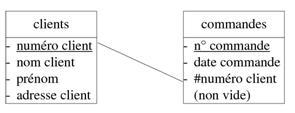
\includegraphics[width=0.7\linewidth]{schema_relationnel.jpg}
  \end{center}
\end{frame}

%\subsection{Traduction d'un modèle conceptuel en un modèle relationnel}

\begin{frame}
  \frametitle{Traduction d'un MCD en un MLDR}
  \begin{itemize}
    \item Pour traduire un MCD en un MLDR, il suffit d'appliquer cinq règles:
      \begin{enumerate}
        \item Traduction d'une entité
        \item Traduction d'une association binaire $1:n$
        \item Traduction d'une association binaire $n:m$
        \item Traduction d'une association binaire $1:1$
        \item Traduction d'une association non binaire
      \end{enumerate}
  \end{itemize}
\end{frame}

\begin{frame}
  \frametitle{Notations}
  \begin{itemize}
    \item Une association binaire est de type :
      \begin{itemize}
        \item $1 : 1$ (un à un) : si aucune des deux cardinalités maximales n'est $n$
        \item $1 : n$ (un à plusieurs) : si une des deux cardinalités maximales est $n$
        \item $n : m$ (plusieurs à plusieurs) : si les deux cardinalités maximales sont $n$
      \end{itemize}
    \item Un schéma relationnel ne peut faire la différence entre $0,n$ et $1,n$
    \item Par contre, il peut la faire entre $0,1$ et $1,1$
  \end{itemize}
\end{frame}

\begin{frame}
  \frametitle{Règle 1: Entité}
  \begin{itemize}
    \item Une entité devient une table:
      \begin{itemize}
        \item Les attributs deviennent les colonnes
        \item L'identifiant constitue la clé primaire de la table
      \end{itemize}
    \item Exemple :\\ L'entité article devient :\\\texttt{articles(\underline{numéro article}, désignation, prix unitaire de
      vente)}
  \end{itemize}
\end{frame}

\begin{frame}
  \frametitle{Règle 2 : Association binaire $1:n$ (1)}
  \begin{itemize}
    \item \texttt{fournisseurs(\underline{numero fournisseur}, nom contact, numero téléphone contact)}
    \item \texttt{livraisons(\underline{numero livraison}, date de livraison, nom livreur, \#numero fournisseur \text{(non
      vide)})}
  \end{itemize}
  \begin{center}
    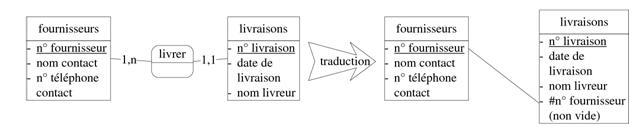
\includegraphics[width=0.9\linewidth]{traduction_1n.jpg}
  \end{center}
\end{frame}

\begin{frame}
  \frametitle{Règle 2 : Association binaire $1:n$ (2)}
  \begin{itemize}
    \item Une association binaire de type $1 : n$ disparaît:
      \begin{itemize}
        \item Au profit d'une clé étrangère dans la table côté $0,1$ ou $1,1$ qui référence la clé primaire de l'autre table
        \item Cette clé étrangère ne peut pas recevoir la valeur vide si la cardinalité est $1,1$
      \end{itemize}
    \item Il ne devrait pas y avoir d'attribut dans une association de type $1 : n$, s'il en reste, ils
      glissent vers la table côté 1.
  \end{itemize}
\end{frame}

\begin{frame}
  \frametitle{Règle 3 : Association binaire $n:m$ (1)}
  \begin{itemize}
    \item \texttt{lignes de commande(\underline{\#numero commande, \#numero article}, quantité commandée)}
  \end{itemize}
  \begin{center}
    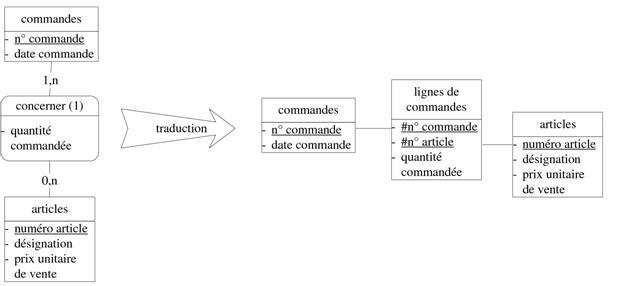
\includegraphics[width=0.9\linewidth]{traduction_nm.jpg}
  \end{center}
\end{frame}

\begin{frame}
  \frametitle{Règle 3 : Association binaire $n:m$ (2)}
  \begin{itemize}
    \item Une association binaire de type $n : m$ devient une table:
      \begin{itemize}
        \item La clé primaire est composée de deux clés étrangères (qui référencent les deux clés primaires
          des deux tables en association)
        \item Les attributs de l'association deviennent des colonnes de cette nouvelle table
      \end{itemize}
  \end{itemize}
\end{frame}

\begin{frame}
  \frametitle{Règle 4 : Association binaire $1:1$ (1)}
  \begin{itemize}
    \item \texttt{services(\underline{numero service}, nom service, \#numéro employé \text{(non vide, unique)})}
    \item \texttt{employés(\underline{numéro employé}, nom)}
  \end{itemize}
  \begin{center}
    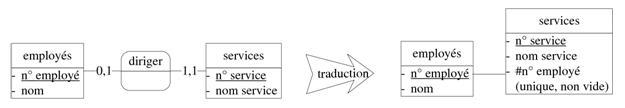
\includegraphics[width=0.9\linewidth]{traduction_11.jpg}
  \end{center}
\end{frame}

\begin{frame}
  \frametitle{Règle 4 : Association binaire $1:1$ (2)}
  \begin{itemize}
    \item Une association binaire de type $1 : 1$ est :
      \begin{itemize}
        \item Traduite comme une association binaire de type $1 : n$
        \item En plus, la clé étrangère se voit imposer une contrainte d'unicité
      \end{itemize}
    \item Si les associations fantômes ont été éliminées, il devrait y avoir au moins un côté de cardinalité
      $0,1$. C'est alors dans la table du côté opposé que doit aller la clé étrangère.
    \item Si les deux côtés sont de cardinalité $0,1$ alors la clé étrangère peut être placée indifféremment
      dans l'une des deux tables.
  \end{itemize}
\end{frame}

\begin{frame}
  \frametitle{Règle 5 : Association non binaire (1)}
  \begin{center}
    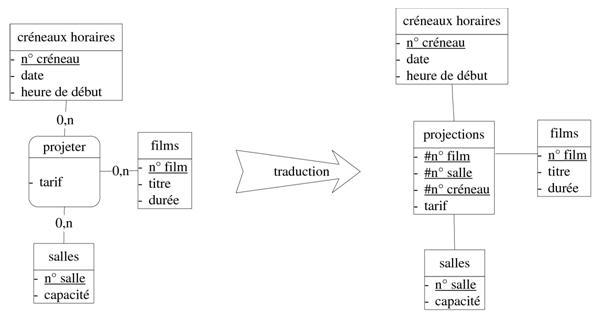
\includegraphics[width=0.9\linewidth]{traduction_non_binaire.jpg}
  \end{center}
\end{frame}

\begin{frame}
  \frametitle{Règle 5 : Association non binaire (2)}
  \begin{itemize}
    \item Une association non binaire est traduite par une table supplémentaire :
      \begin{itemize}
        \item La clé primaire est composée d'autant de clés étrangères que d'entités en association
        \item Les attributs de l'association deviennent des colonnes de cette nouvelle table
      \end{itemize}
  \end{itemize}
\end{frame}

%\subsection{Compléments}

\begin{frame}
  \frametitle{Optimisation (1)}
  \begin{itemize}
    \item L'optimisation des performances en temps de calcul se fait toujours au détriment de l'espace mémoire
      consommé
    \item Dans le pire des cas, réduire les temps de réponse consiste à dé-normaliser volontairement le
      système d'information, avec tous les risques d'incohérence et les problèmes de gestion que cela
      comporte
    \item Le conseil le plus précieux, en matière d'optimisation, est de ne jamais optimiser \emph{a priori},
      mais toujours \emph{a posteriori} :
    \item[$\ra$] C'est-à-dire en réponse à une lenteur que le SGBDR n'est pas capable de résoudre tout seul
    \item Il convient de mesurer le gain de toute optimisation manuelle en effectuant des tests
      (chronométrages avant/après) sur un volume de données significatif et de préférence en exploitation
  \end{itemize}
\end{frame}

\begin{frame}
  \frametitle{Optimisation (2)}
  \begin{itemize}
    \item Pour les bases de données relationnelles, l'optimisation peut passer par :
      \begin{itemize}
        \item L'ajout d'index aux tables (au minimum sur les colonnes clés primaires et clés étrangères):
          \begin{itemize}
            \item Ces index consomment de l'espace mémoire supplémentaire
            \item La base de données reste normalisée
          \end{itemize}
        \item L'ajout de colonnes calculées ou de certaines redondances :
          \begin{itemize}
            \item Permet d'éviter des jointures coûteuses
            \item La base est dé-normalisée
            \item Il faut alors veiller à ce que la cohérence entre les colonnes soit respectée (déclencheurs
              ou code client)
          \end{itemize}
        \item La suppression des contraintes :
          \begin{itemize}
            \item D'unicité, de clé étrangère, etc.
            \item L'intégrité des données doit être assurée par le code client
          \end{itemize}
      \end{itemize}
  \end{itemize}
\end{frame}

\begin{frame}
  \frametitle{Optimisation : Exemple}
  \begin{itemize}
    \item La table commandes peut être supprimée et la date de commande est alors ajoutée à la table lignes de
      commandes
  \end{itemize}
  \begin{center}
    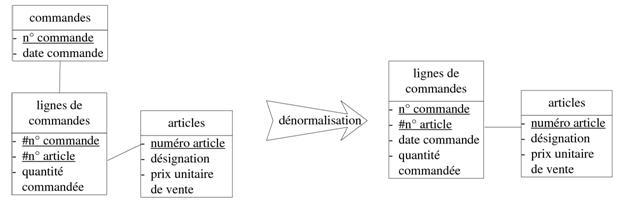
\includegraphics[width=0.9\linewidth]{optimisation.jpg}
  \end{center}
  \begin{itemize}
    \item On renonce donc à la troisième forme normale :
      \begin{itemize}
        \item La date de commande est répétée autant de fois qu'il y a de lignes dans la commande
        \item Mais on évite une jointure coûteuse en temps de calcul lors des requêtes SQL
      \end{itemize}
  \end{itemize}
\end{frame}

\begin{frame}
  \frametitle{Héritage (1)}
  \begin{itemize}
    \item Factorisation des attributs communs à plusieurs entités au sein d'une entité mère
  \end{itemize}
  \begin{center}
    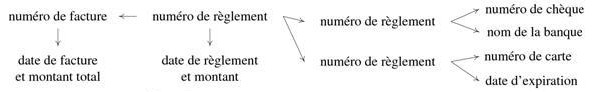
\includegraphics[width=0.9\linewidth]{heritage_1.jpg}
  \end{center}
  \begin{itemize}
    \item Exemple :
      \begin{itemize}
        \item Factures de paiement par chèque ou par carte
        \item On souhaite connaître pour chaque règlement la \emph{date} et le \emph{montant}
      \end{itemize}
  \end{itemize}
\end{frame}

\begin{frame}
  \frametitle{Héritage (2)}
  \begin{center}
    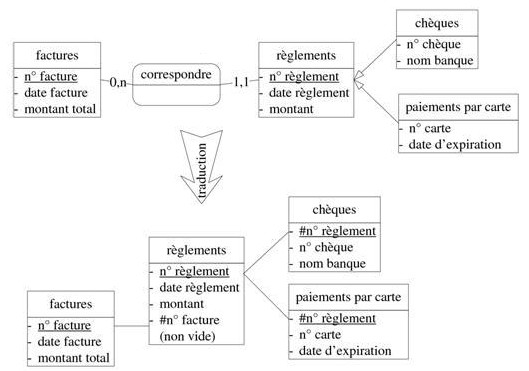
\includegraphics[width=0.7\linewidth]{heritage_2.jpg}
  \end{center}
  \begin{itemize}
    \item[$\ra$] Une entité générique règlements et deux entités spécialisées chèques et paiements par carte
    \item Lien d'héritage représenté par une flèche creuse\\ 
       (ce lien remplace une association de type $1 : 1$)
  \end{itemize}
\end{frame}

\begin{frame}
  \frametitle{Héritage (3)}
  \begin{itemize}
    \item Les deux sous-entités de l'entité règlements ont des attributs propres mais pas d'identifiant
      propre
    \item Il ne faut pas voir d'héritage à chaque fois que l'on peut dire « est un » :\\
      il faut en plus que l'entité mère ne possède que les attributs communs de ses entités filles
    \item La traduction des sous-entités au niveau logique relationnel fait intervenir une clé primaire
      identique à celle de l'entité mère, mais dans les sous-entités la clé primaire est aussi étrangère
  \end{itemize}
\end{frame}

\begin{frame}
  \frametitle{Héritage et informations complémentaires}
  \begin{itemize}
    \item L'héritage est également utile pour stocker des informations complémentaires
  \end{itemize}
  \begin{center}
    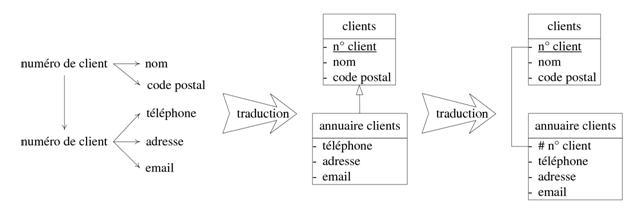
\includegraphics[width=0.9\linewidth]{heritage_informations_complementaires.jpg}
  \end{center}
  \begin{itemize}
    \item Exemple :
      \begin{itemize}
        \item Table clients avec numéro, nom et code postal
        \item Ajout de trois colonnes mais il y a déjà des valeurs saisies
        \item[$\ra$] Une nouvelle table permet de gagner de la place
      \end{itemize}
  \end{itemize}
\end{frame}

\begin{framentitle}{Héritage et contraintes (1)}
    \begin{itemize}
       \item Il est possible de préciser sur le modèle conceptuel des
            contraintes sur l'héritage :
            \begin{itemize}
                \item Exclusivité ($X$): équivaut à un «~OU exclusif~». On est l'une,
                    l'autre ou aucune, mais pas les deux à la fois.
                \item Totalité ($T$) : équivaut à un «~OU~». On est l'une,
                    l'autre, les deux, mais pas aucune des deux.
                \item Partition ($XT$) : totalité + exclusivité. On est l'une ou
                    l'autre (et donc ni les deux, ni aucune des deux).
                \item Vide : on est l'une, l'autre, les deux ou aucune des deux.
            \end{itemize}
    \end{itemize}
\end{framentitle}

\begin{framentitle}{Héritage et contraintes (2)}
    \begin{center}
    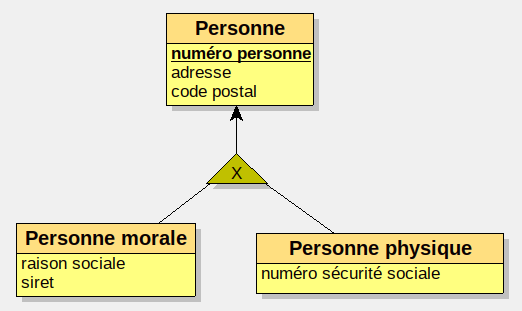
\includegraphics[width=.8\textwidth]{heritage_x.png}
    \end{center}
    \begin{itemize}
        \item Exclusivité ($X$): équivaut à un «~OU exclusif~».\\On est l'une,
            l'autre ou aucune, mais pas les deux à la fois.
    \end{itemize}
\end{framentitle}

\begin{framentitle}{Héritage et contraintes (3)}
    \begin{center}
    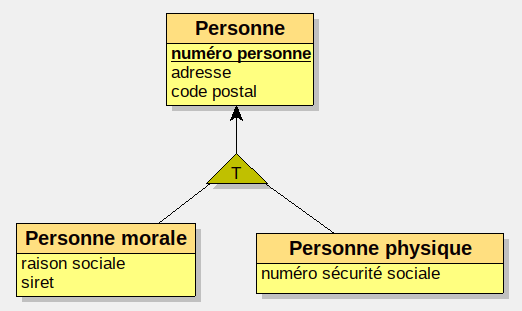
\includegraphics[width=.8\textwidth]{heritage_t.png}
    \end{center}
    \begin{itemize}
        \item Totalité ($T$) : équivaut à un «~OU~».\\On est l'une, l'autre, les
            deux, mais pas aucune des deux.
    \end{itemize}
\end{framentitle}

\begin{framentitle}{Héritage et contraintes (4)}
    \begin{center}
    \includegraphics[width=.8\textwidth]{heritage_xt.png}
    \end{center}
    \begin{itemize}
        \item Partition ($XT$) : totalité + exclusivité.\\On est l'une ou l'autre
            (et donc ni les deux, ni aucune des deux).
    \end{itemize}
\end{framentitle}

\begin{framentitle}{Héritage et contraintes (5)}
    \begin{center}
    \includegraphics[width=.8\textwidth]{heritage_vide.png}
    \end{center}
    \begin{itemize}
        \item Vide :\\On est l'une, l'autre, les deux ou aucune des deux.
    \end{itemize}
\end{framentitle}



\end{document}

